\documentclass[10pt, aspectratio=169]{beamer}

\usepackage{tgschola}
\usepackage{subfig}
\usepackage{float}
\usepackage{wrapfig}

\title{Brain Tumor Detection using Machine Learning Models}

\subtitle{B.Sc. Semester VI Project \newline Department of Computer Science, Gurudas College}

\usetheme{Madrid}

\date{}

\author[Rajarshi, Bhargav, Soptorshi, Brahmajit] {
	Bhargav Basu \texorpdfstring{\\} \and
	Soptorshi Bhattacharjee \texorpdfstring{\\} \and
	Brahmajit Das \texorpdfstring{\\} \and
	Rajarshi Sardar
}

\institute[Gurudas College]{Gurudas College, Calcutta University}

\begin{document}

	\frame{\titlepage}

	\begin{frame}
		\frametitle{Overview}
		\tableofcontents
	\end{frame}

	\section{Motivation}
	\begin{frame}
		\frametitle{Motivation}

		The motivation is to develop a software with better segmentation
		capability for use in medical imaging to detect diseases like brain
		tumor. Image segmentation has been identified as the key problem of
		medical image analysis and remains a popular and challenging area of
		research. Image segmentation is increasingly used in many clinical and
		research applications to analyze medical imaging datasets; which
		motivated us to present a snapshot of dynamically changing field of
		medical image segmentation.

		\vspace{0.5cm}

		The motivation of this work is to increase patient safety by providing
		better and more precise data for medical decision.
	\end{frame}

	\section{Domain Description}

	\begin{frame}
		\frametitle{Domain Description}

		\begin{itemize}
			\item
			\textbf{Neurological Examination}: It is a series of test to measures
			the function of the patients nervous system and also his/her physical
			and mental alertness. \pause
			\item
			\textbf{Machine Learning}: Machine learning approaches address these
			problems by mainly using hand-crafted features (or pre-defined
			features). \pause
		   \item
		   \textbf{Brain Scans}: Brain scan is a picture of the internal
		   structure of the brain. A specialized machine takes a scan in the
		   same way as a digital camera takes a photograph.
		\end{itemize}
	\end{frame}

	\section{Background}

	\begin{frame}
		\frametitle{Background}

		We propose the use of ML algorithms to overcome the drawbacks of
		traditional classifiers. We investigate and compare the performance of
		various machine learning models, namely \textbf{CNN}, \textbf{VGG 16}
		and \textbf{ ResNet 50 }; implemented using the frameworks Tensorflow
		and fast.ai.
	\end{frame}

	\section{Methodology}

	\begin{frame}
		\frametitle{Methodology}

		\vspace{-2.5cm}

		\begin{figure}[h]
			\centering
			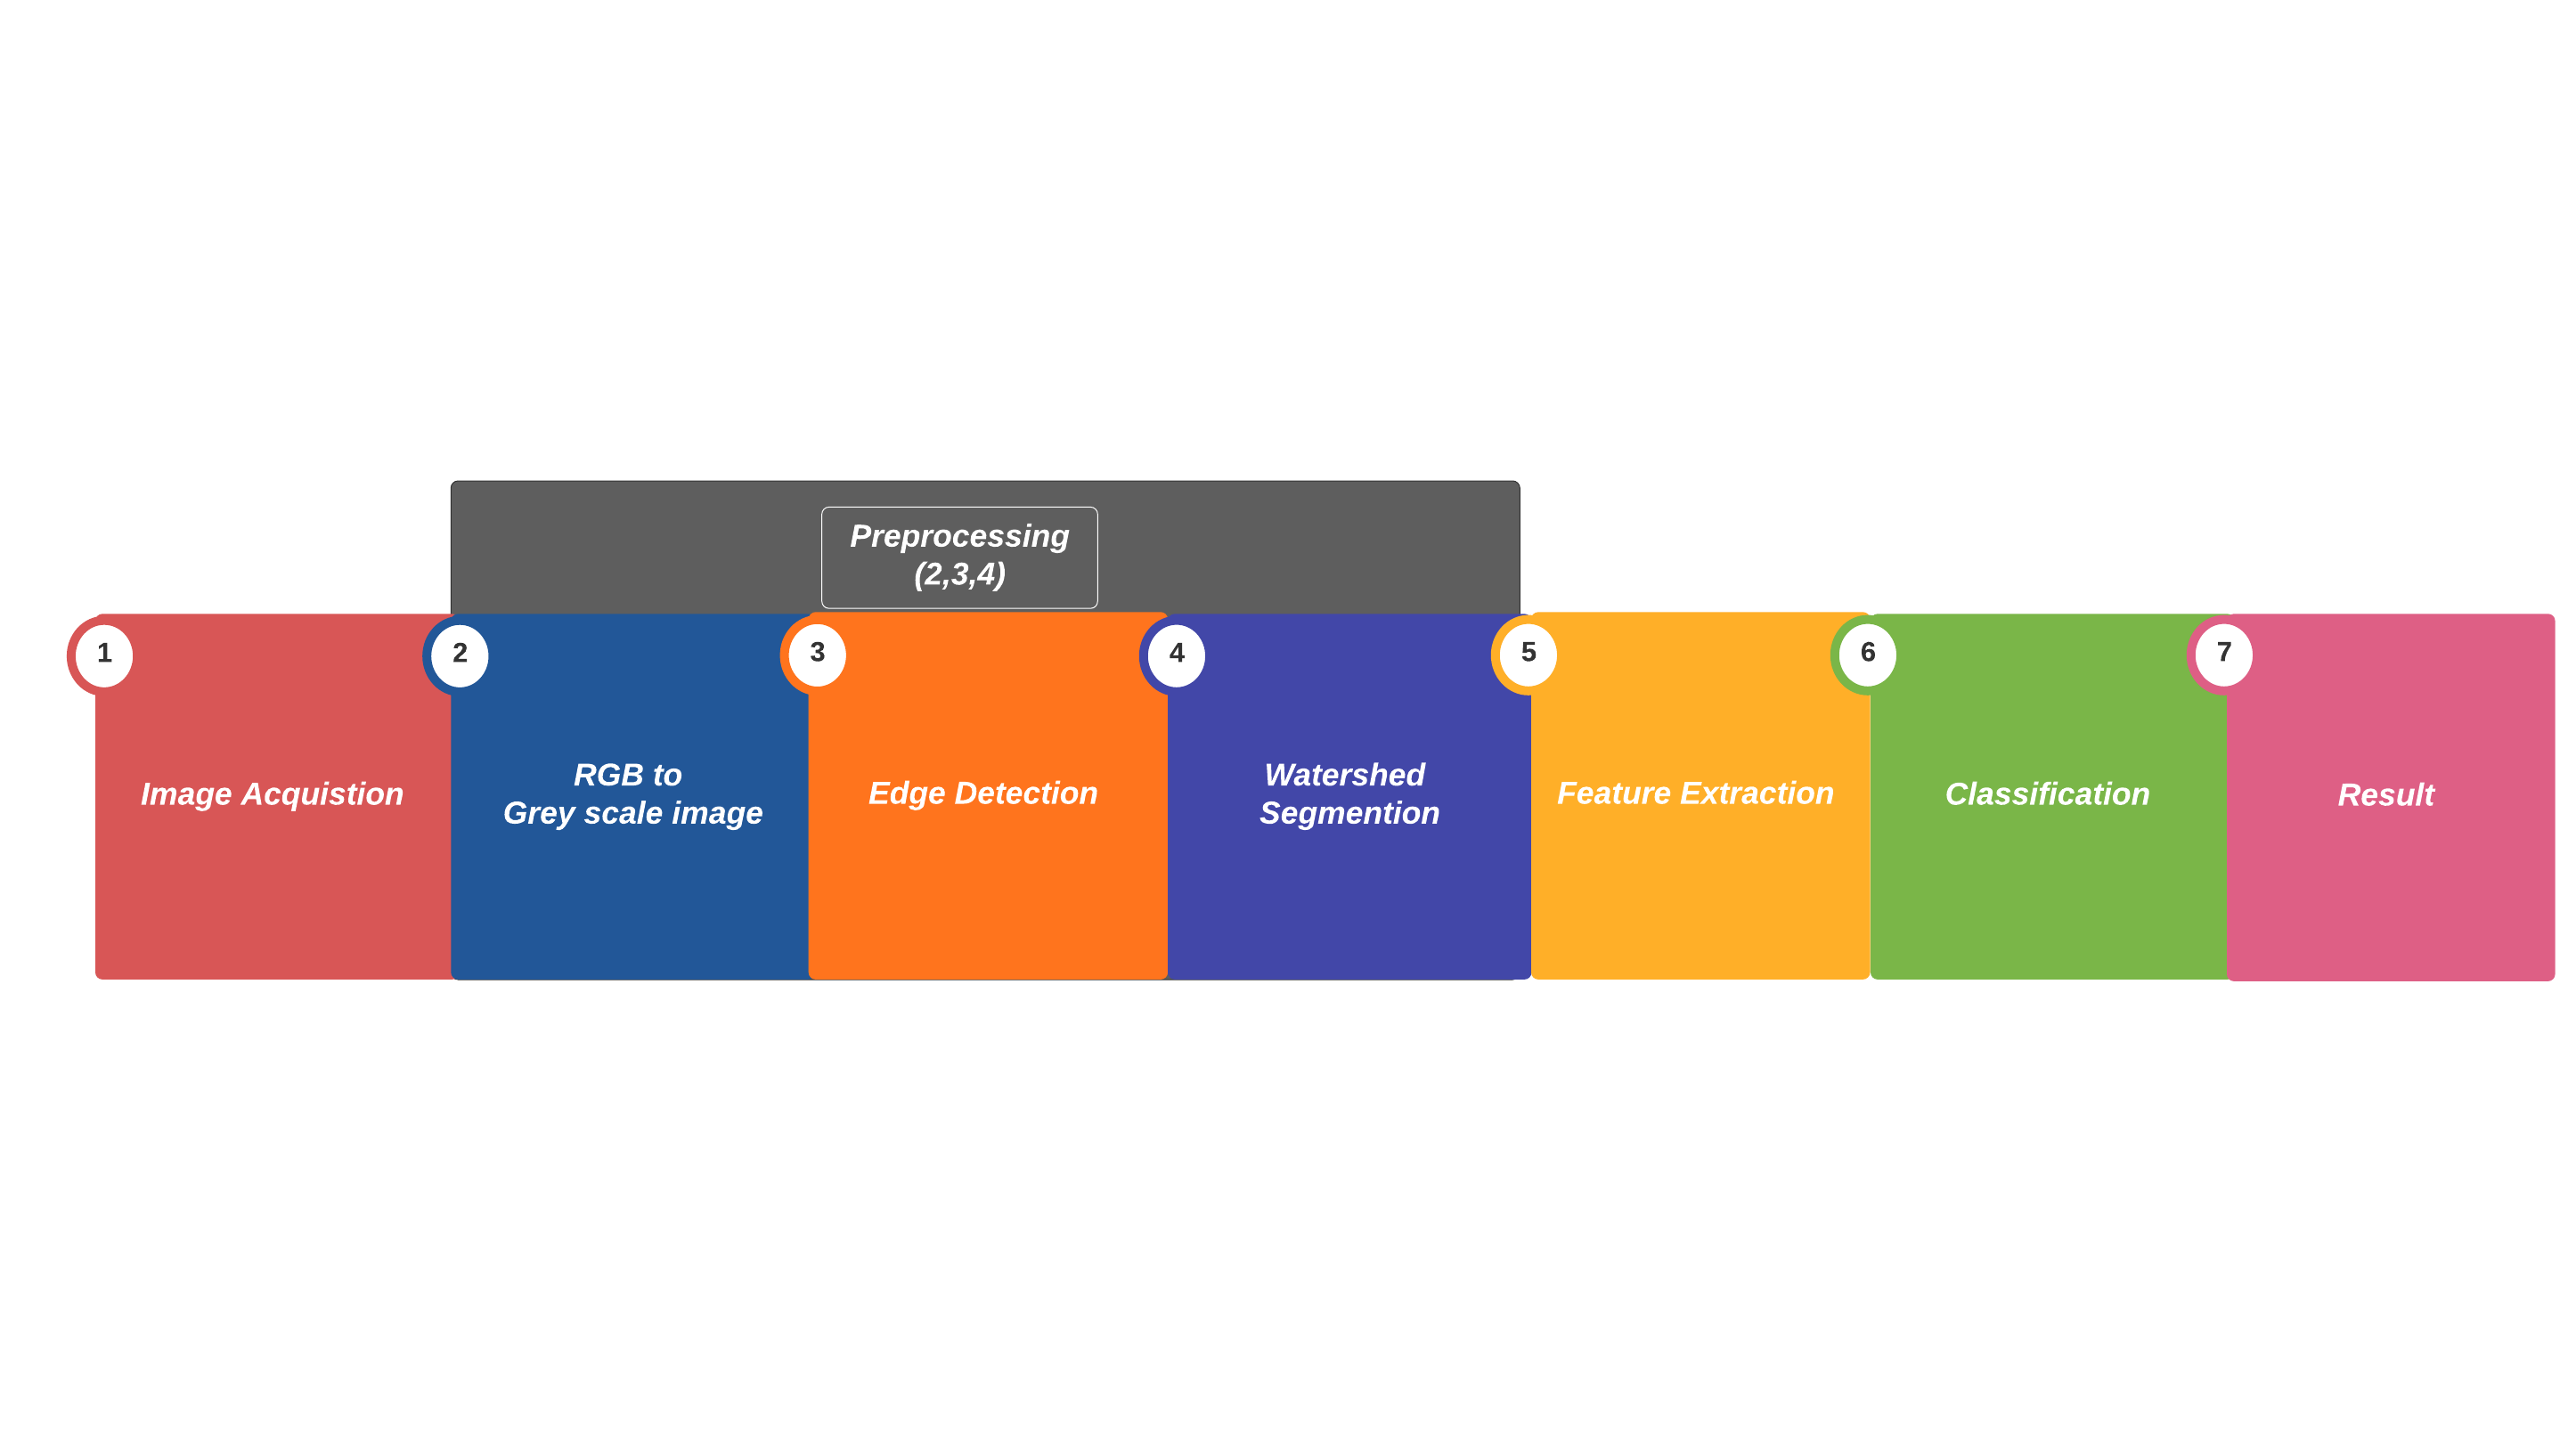
\includegraphics[width=\linewidth]{imgs/flowchart}
			\caption{Proposed Methodology}%
			\label{fig:prop_methodology}
		\end{figure}

	\end{frame}

	\subsection{Image Acquisition}

	\begin{frame}
		\frametitle{Methodology}
		\framesubtitle{Image Acquisition}
		The MRI brain images are acquired and are given as input to
		pre-processing stage.

		\begin{figure}[H]
			\centering
			\subfloat[MRI scan shown no presence of tumor]
			{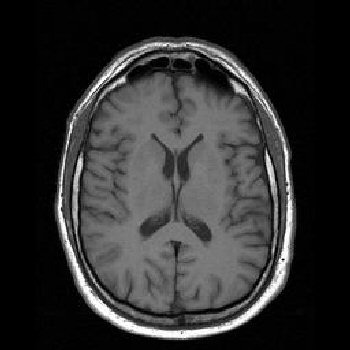
\includegraphics[width=0.25\textwidth]
			{imgs/pred1.jpg}\label{scan2}}
			\hspace{0.2cm}
			\subfloat[MRI scan of a tumorous cell]
			{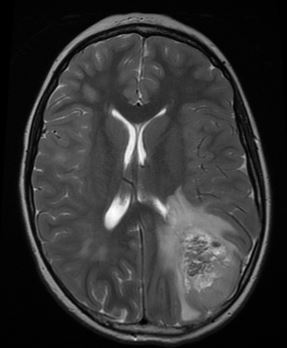
\includegraphics[width=0.2\textwidth]
			{imgs/Y100.JPG}\label{scan1}}
			\caption{MRI Scans}
			\label{MRIScans}
		\end{figure}
	\end{frame}

	\subsection{Preprocessing}

	\begin{frame}
		\frametitle{Methodology}
		\frametitle{Preprocessing}

		Preprocessing is needed as it provides improvement in image data which
		enhances some of the image features which are important for further
		processing.

		\vspace{1cm}

		Preprocessing includes:

		\begin{itemize}
			\item Binarization
			\item Filtering
			\item Edge Detection
			\item Segmentation
		\end{itemize}
	\end{frame}

	\begin{frame}
		\begin{figure}[ht]
			\centering
			\subfloat[Original Image]
			{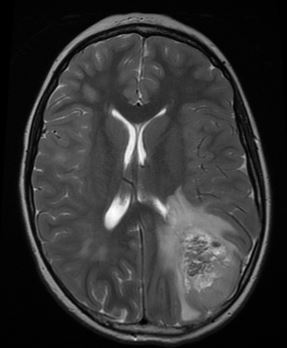
\includegraphics[width=0.2\linewidth]
			{imgs/Y100.JPG}\label{original}}
			\hspace{0.5cm}
			\subfloat[Filtered Imaage]
			{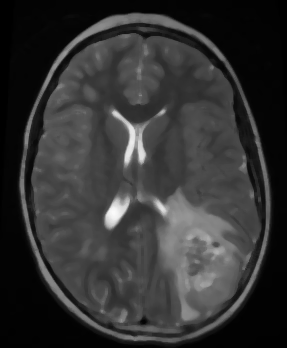
\includegraphics[width=0.2\linewidth]
			{imgs/median_filtering.png}\label{smooted image}}
			\hspace{0.5cm}
			\subfloat[Edge Detection]
			{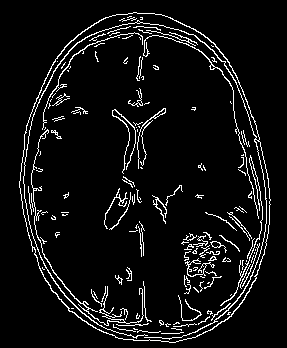
\includegraphics[width=0.2\linewidth]
			{imgs/edges_detection.png}\label{edge detection}}
			\hspace{0.5cm}
			\subfloat[Segmentation]
			{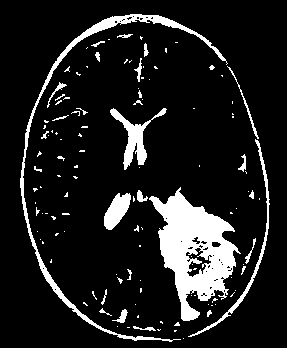
\includegraphics[width=0.2\linewidth]
			{imgs/segmentation.png}\label{segmentation}}
			\caption{preprocessing operations}
			\label{Preprocessing Operations}
		\end{figure}
	\end{frame}
\end{document}
